% Bias in Candidate Sourcing
\documentclass[man]{apa7}

\usepackage[american]{babel}

\usepackage{csquotes}

\usepackage[style=apa,sortcites=true,sorting=nyt,backend=biber]{biblatex}

\usepackage{titlesec}

\usepackage{setspace}

\usepackage{enumitem}

\usepackage{endnotes}

\usepackage[longtable]{multirow}

\usepackage[flushleft]{threeparttable}

\DeclareLanguageMapping{american}{american-apa}
\addbibresource{bibliography.bib}

\graphicspath{{'./Users/nyxinsane/Documents/Work - UvA/Automating Equity/Study 1/Study1_Code/data/plots/'}}

\title{Bias in Candidate Sourcing Communication:\\
Investigating Stereotypical Gender- And Age-Related Frames in Online Job Advertisements at the Sectoral Level}
\shorttitle{Bias in Candidate Sourcing Communication}

\authorsnames[1,1,{2},1,1]{Noon M.F. Abdulqadir, Anne Kroon, Martine van Selm, Margot van der Goot, and Rens Vliegenthart}
\authorsaffiliations{{Amsterdam School of Communication Research (ASCoR)},
{Erasmus School of History, Culture and Communication}}

\leftheader{Noon et al.}

\abstract{Studies show the extent to which job advertisements contain stereotypical wordings correlates with the level of segregation in an occupational domain. However, limited research links the framing of job ads to social category-based occupational segregation at the macro-sectoral level. Guided by the stereotype content model, we operationalize stereotypical warmth and competence-related frames in candidate sourcing communication and investigate their presence in job ads from occupational sectors with varying gender and age segregation. Automated content analysis was conducted on a dataset of online job ads sentences (\textit{n}=307154). Results indicate warmth-related frames are most observed in ads from female (vs. male) and younger (vs. older and mixed-age) dominated sectors. Conversely, competence-related frames are most observed in ads from male (vs. female and mixed-gender) and older (vs. younger and mixed-age) dominated sectors. Taken together, we present an operationalization of stereotypical warmth- and competence-related frames in early employer communication and posit that social categorization framing may be at play.}

\keywords{Stereotype content model, social categorization frames, horizontal occupational segregation, automated content analysis}

\authornote{
   \addORCIDlink{Noon M.F. Abdulqadir}{https://orcid.org/0000-0002-6243-9241}

   \addORCIDlink{Anne Kroon}{https://orcid.org/0000-0001-7600-7979}

   \addORCIDlink{Martine van Selm}{https://orcid.org/0000-0001-9188-4021}

   \addORCIDlink{Margot van der Goot}{https://orcid.org/0000-0001-6904-6515}

   \addORCIDlink{Rens Vliegenthart}{https://orcid.org/0000-0003-2401-2914}

   \qquad We have no conflicts of interests to disclose.

   \qquad Correspondence concerning this article should be addressed to Noon Abdulqadir, Postbus 15791, 1001 NG Amsterdam. Email: noon.abdulqadir@uva.nl

   \qquad \textbf{Suggested citation:} Noon, M. A., Kroon, A. C., van Selm, M., van der Goot, M., and Vliegenthart, R. (2021). Bias in Candidate Sourcing Communication: Investigating Stereotypical Gender- and Age-Related Frames of Online Job Advertisements at the Sectoral Level.}

\begin{document}
\maketitle
Scholars have long documented the influence of interpersonal bias in candidate recruitment, particularly with regard to job seekers’ gender and age \parencite{beattie_possible_2012, heilman_gender_2012, paleari_when_2019}. This influence is observable during active candidate sourcing where job advertisements represent the first touchpoint in employer communication \parencite{RynesS.1989}. These job ads can signal essential value-related information about an organization \parencite{de_cooman_portraying_2012} but can also determine the pool of potential candidates who apply for an advertised position and reinforce existing interpersonal biases. On the micro-level, job ads and the HR decisions that dictate their content are informed by the type of candidate employers explicitly or implicitly envision as “ideal” for a position \parencite{kelly_gendered_2010}. \Textcite{van_selm_search_2021}, for instance, found that job ads targeting older workers contained frames consistent with general stereotypes of older individuals. On the meso-level, the content of job ads can also reflect the level of segregation (homogeneity), or lack thereof (heterogeneity), in an occupation. As \Textcite{gaucher_evidence_2011} found, job ads from traditionally male-dominated occupations such as engineer, plumber, and security guard tend to contain terms such as competitive, leader, ambitious, and similar wordings that are culturally related to masculinity, consequently making such ads less appealing to female candidates.

Thus far, limited research has explored the relationship between the content of job advertisements and macro-level occupational segregation, i.e., at the sectoral level, demarcated specifically by social category composition \parentext{with the exception of \nptextcite{grabhorn_social_2006} as cited in \nptextcite{clarke2020GenderStereotypesGenderTyped}}. Although career changes across sectors are more common than ones across occupations \parencite{carrillo-tudela_extent_2016}, workers generally tend to stay within social category-typed sectors due to a backlash effect \parencite{fritsch_horizontal_2020}. For example, a female social worker making a career change from the Health and social work activities sector may be more likely to go into the Education or Government and care sectors, both highly female-dominated. Similarly, an older logistics manager in the Transportation and storage sector may more readily consider a career as a production manager in the Manufacturing sector than an ICT-manager in the younger-typed Information and communication sector. Sectoral segregation demarcated based on social category composition may thus be more persistent and present a higher social barrier to entry than segregation demarcated based on other occupational factors, thus becoming key to understanding possible inequity in candidate sourcing.

Given this, the present study makes three main contributions. First, it investigates candidate sourcing in Dutch intranational sectors that are heterogeneous and homogenous in gender and age composition, i.e., female- and male-dominated (vs. mixed-gender sectors) and older worker- and younger worker-dominated (vs. mixed-age sectors respectively) \ref{table:10}. Informed by framing theory and the stereotype content model, we examine the extent to which framed gender- and age-related stereotypes are present in online job ads from heterogeneous and homogenous sectors. Second, it presents a systematic operationalization of broad-level gender- and age-related stereotypical frames in job ads. Employing the social categorization framing hypothesis \parencite{Yang2015a}, we adopt the conceptualization of pancultural and generalizable warmth- and competence-related social category stereotypes put forth in the SCM \parencite{fiske_model_2002}. Third, we utilize a rigorous automated content analysis method that serves as an exemplary analysis of how to detect biases in texts. This study thus seeks to answer the question: \textit{to what extent are job advertisements from social category-typed occupational sectors framed in terms of warmth- and competence-based gender and age stereotypes?}

\subsection{Framing Theory and Stereotypical Frames}
\label{framing}
Framing a message constrains its audiences to desired and meaningful interpretations by directing attention to information judged to be important by the message sender. Frames make salient some aspects or subset of possible considerations about a subject over others \parencite{entman_framing_1993}, typically through strategic “selection, emphasis, exclusion, and elaboration” \parencite[p. 10] {reese_framing_2001}. Within framing theory, stereotypes are a powerful framing device underscored by culturally-embedded implicit reasoning devices \parencite{van_gorp_where_2005}, i.e., they draw on and activate culturally shared (consensual) cognitive schemata. In their capacity as framing devices, stereotypes draw attention to a particular assessment of social categories, their roles, and their distance from the reader, thus stereotypes may come to define a frame.

Expounding on the use of stereotypes in framing, \parencite{Yang2015a} presents a typology of stereotypical frame genres differentiated through their effects on cognition and the pathway by which they make salient the perceived social distance between categories, i.e., degree of emphasis on the self-to-other differences. \textit{Social categorization frames} in particular are germane to the current study as their usage centers around ownership of cultural objects such as social roles or certain jobs and occupational sectors. By emphasizing the belongingness of cultural objects to select social categories, social categorization frames activate distinct social identities, otherization, and make salient the social distance between social categories. This frame genre thus conveys the reasoning that “certain groups are outgroups and their members are not qualified for ingroup activities” \parencite[p. 261]{Yang2015a}. Likewise, social categorization frames may activate self-stereotyping and lead to ingroup members assuming the characteristics stereotypically associated with their category, increasing conformity and deindividuation \parencite{brown2003BlackwellHandbookSocial}.

Social categorization frames are also applied differently to different categories depending on whether they are dominant or non-dominant in a domain. When addressing dominant social categories, emphasis is placed on ingroup characteristics and their complementarity to features of the cultural object. When addressing outgroups, the information also tends to be stereotype-consistent, however, the emphasis is on the mismatch between the cultural object and the categories’ characteristics. Examples of social categorization framing include female political candidates being framed as intruders and a novelty in political races by the news media \parencite{meeks_all_2013, sullivan_1984_1989} and older individuals depicted as a burden due to their employment statuses, healthcare costs, and social benefits allowances \parencite{ng_evaluating_2012}. Applied to job ads wherein messages are targeted to perceived ideal candidates, frames in job ads from sectors that are “owned” by a single social category, i.e., from a homogeneous sector, are likely to emphasize stereotypical characteristics perceived as essential to the dominant social category.

\subsection{Stereotype Content Model \parentext{SCM}}
\label{scm}
Examining consensual stereotypes, i.e., stereotypes that are (perceived to be) shared by the wider culture \parencite{fiske_prejudices_2017, gardner1994}, \Textcite{beukeboom_how_2019} describe stereotype content as the “[cognitive] representation people hold about a social category, consisting of beliefs and expectancies about probable behaviors, features, and traits” \pnotecite[9]{beukeboom_how_2019}. The extent to which stereotype content is endorsed depends on the strength of individual essentialist beliefs about the stereotyped category \parencite[for perceived category essentialism and stereotyping, see][]{beukeboom_how_2019}.

Specific stereotypes about both gender and age categories can vary across cultures and within different strata of the same culture. One model that circumvents this barrier is the \textit{stereotype content model} (SCM) as it is suitable for investigating pancultural, superordinate, and broad-level stereotypes. Developed by \Textcite{fiske_model_2002}, the SCM provides a universal principle determining predictors of stereotypes and sets up a framework to comparatively and systematically investigate stereotype content \parencite{kroon_reliable_2018, van_selm_search_2021}. Due to its generalizability and intuitiveness, the SCM has been routinely used by scholars to analyze intergroup communication, media, and text for markers of other- as well as self-stereotyping \parencite{westerhof_filling_2010, white_think_2009}. In recruitment, \Textcite{hofhuis_dealing_2016} relate warmth and competence perceptions to social and task-performance ratings HR managers assigned to job candidates. In textual data analysis, the SCM’s applications have extended into computational research as a framework for stereotype- and bias-detection natural language models \parencite{nicolas2020ComprehensiveStereotypeContent}.

The SCM differentiates pancultural stereotype content along two perceptual dimensions: \textit{warmth} and \textit{competence} \parencite{cuddy_stereotype_2009}. Perceived warmth is related to compassion, kindness, helpfulness, and interpersonal sensitivity whereas perceived competence is associated with self-assertion, leadership, analytical thinking, and independence \parencite[]{bruckmuller_density_2013, Carli2016, hummert_multiple_1990}. The assessments of outgroup members along these two dimensions form the core of social category stereotypes including ingroup self-stereotypes \parencite{hinton_exploring_2019}. According to the SCM, gender groups are social categories that are subject to cross-cultural stereotyping along the dimensions of warmth and competence\endnote{For transgender, genderqueer, and gender-nonconforming individuals, stereotypes vary and are highly dependent on endorsement of gender essentialist beliefs \parencite{Gallagher2020}.} \parencite{fiske_model_2002}. Females (and women generally) are linked to warmth traits but perceived as low in competence whereas males (and men generally) are linked to competence traits but perceived as low in warmth \parencite{Eagly1997, suh_gender_2004}. Different age groups also have associated warmth- and competence-related stereotypes: older individuals are perceived as lacking in competence compared to their younger counterparts but generally rated higher on warmth whereas younger individuals are perceived as lacking in warmth but consistently rated higher on competence \parencite{cuddy_this_2005, van_selm_search_2021}.

\subsubsection{Gender Stereotypes in the Occupational Domain}
The stereotypical attribution of warmth and competence to females and males also form the basis for stereotypes about female and male workers \parencite{froehlich_gender_2020} and is further generalizable to gendered occupational domains. Various studies point to the observability of gendered warmth and competence stereotype differences in diverse contexts and across analytical approaches \parencite{aaldering_political_2020, harmer_are_2017}. \Textcite{smith_power_2019} found that positive attribute assignments to female and male leaders were aligned with the SCM, however, female leaders were more likely to be perceived as exhibiting cold characteristics compared to their male counterparts. These findings implicitly provide evidence for social categorization framing through the \textit{lack of fit} model \parencite[see][]{heilman_gender_2012, horvath_reducing_2016}. Dominant social groups with stereotyped characteristics matching (and seen as essential to) a social role are appraised based on said characteristics whereas non-dominant groups with mismatching stereotyped characteristics are appraised via both characteristics of the social role and the social group – the latter often resulting in unfavorable appraisal.

Particular to occupational segregation, a survey by \Textcite{he_stereotypes_2019} on warmth and competence perception associated with different occupations found a positive correlation between occupational stereotype content and the respective level of gender segregation. Nursing, medical assistance, childcare, and secretarial work were the highest-rated occupations on warmth, and women made up the majority in these occupations: 89.4\%, 90.7\%, 94.9\%, and 94.5\% respectively. Similarly, \Textcite{strinic_occupational_2021}, in a survey using a sample of 130 HR professionals, found that stereotypical perceptions of warmth and competence are in fact attached to occupations.

In light of the reviewed literature, we expect similar differences in the presence of warmth- and competence-related stereotypical frames in job ads at the sectoral level:

\begin{enumerate}[leftmargin=2.5cm, labelsep=0.25cm, align=left, label={\textbf{Hypothesis \arabic*:}}]

\item Job advertisements from female-dominated sectors will include more warmth-related frames when compared to job advertisements from male-dominated sectors \parentext{\textbf{H1a}} or mixed-gender sectors \parentext{\textbf{H1b}}.

\item Job advertisements from male-dominated sectors will include more competence-related frames when compared to job advertisements from female-dominated sectors \parentext{\textbf{H2a}} or mixed-gender sectors \parentext{\textbf{H2b}}.

\end{enumerate}

\subsubsection{Age Stereotypes in the Occupational Domain}
Stereotypical attribution of warmth and competence to workers from different age groups also aligns with the general stereotypes of individuals in those categories. In a frame analysis study of Dutch media texts published over the span of six years, \Textcite{kroon_reliable_2018} found that both corporate and news media portray older workers as trustworthy, involved, and committed (warmth characteristics) but lacking in aptitudes related to productivity, adaptability, and technological skills (competence characteristics). \Textcite{krings_stereotypical_2011} also found that good-naturedness, amicability, benevolence, and sincerity formed the content of warmth-related stereotypes for older workers while capability, efficiency, and skill formed the content of competence-related stereotypes for younger workers.

In job ads, different contextual factors seem to be at play. \Textcite{van_selm_search_2021} found hard abilities requirements for general job seekers (e.g., business operations, leadership, and professional development abilities) were more pronounced compared to soft abilities requirements for older workers (e.g., customer service ability). This emphasis on competence over warmth was also noted in a study by \Textcite{Abraham2015} where role congruity between a job’s age type and an older candidate’s stereotyped characteristics did not increase older candidate selection. Findings point to an undervaluing of older workers’ warmth characteristics and indicate warmth-primacy – wherein proneness to evaluate others positively is predicted primarily by warmth perceptions \parencite{cuddy2008WarmthCompetenceUniversal, ponsi_influence_2016} – functions differently in the context of age-typed recruitment. Moreover, de-emphasis on warmth may signal a cleave between interpersonal and occupational stereotypes as it pertains to age, or that the characteristics of older workers such as higher knowledge-sharing motivations confer on them perceptions of competence \parencite{burmeister_understanding_2020}.

Literature thus suggests that when comparing job ads from older-worker-dominated and younger-worker-dominated sectors, the presence of competence-related frames may be more relevant than the absence of warmth-related frames in determining whether bias against older workers (or in favor of younger workers) may exist. Notwithstanding, as social stereotypes about older individuals form the basis for older-worker stereotypes, we expect:

\begin{enumerate}[leftmargin=2.5cm, labelsep=0.25cm, align=left, label={\textbf{Hypothesis \arabic*:}}]
\setcounter{enumi}{2}

\item Job advertisements from sectors dominated by older workers will include more warmth-related frames when compared to job advertisements from sectors dominated by younger workers \parentext{\textbf{H3a}} or mixed-age sectors \parentext{\textbf{H3b}}.

\item Job advertisements from sectors dominated by younger workers will include more competence-related frames when compared to job advertisements from sectors dominated by older workers \parentext{\textbf{H4a}} or mixed-age sectors \parentext{\textbf{H4b}}.

\end{enumerate}

\section{Method}
\label{method}
To assess the presence of warmth- and competence-related frames in job ads, we employ a two-stage approach. First, we use a quantitative method of manual content analysis to categorize job ads based on these two dimensions. Next, we use the annotations from this manual analysis to train classifiers, which enables automated labeling of the remaining job ads in our sample.

\subsection{Data Collection and Sample}
Job ads were collected based on searches for sector-keywords from three online job search platforms: LinkedIn.nl, Indeed.nl, and Glassdoor.nl\endnote{These platforms were chosen as Indeed.nl was the most popular job search board in the Netherlands with a share of 44\% active job seekers followed by LinkedIn with 35\% whereas Glassdoor was popular with employers and provided English language support \parencite{intelligencegroup2020Top10Job}}. Sector designations and search-keywords were obtained from the International Standard Industrial Classifications \parencite[SBI;][]{centraal_bureau_voor_de_statistiek_standard_2018}. Some of the original 19 SBI sector titles were a combination of multiple independent sector designations, e.g., “agriculture and industry”. These sector titles returned imprecise search results and were thus divided into distinct sector search-keywords and the resultant list was supplemented with data from the more detailed codes and the Dutch Labour Force Survey \parencite{centraal_bureau_voor_de_statistiek_dutch_2021}. All 19 sectors were included, and 99 sector-keywords were used (excluding pluralization and alternative spellings). Table 10 in Appendix A provides an overview of sector classifications, used search-keywords, and sector composition.

All scraping, preprocessing, and analysis scripts used in this paper were written using Python 3.10 (GITHIB REPOSITORY LINK BLINDED FOR PEER REVIEW). Data collection ran from November 2020 until April 2021. Duplicate, malformed, and non-English language job ads were filtered. The final sample comprised 16134 job ads containing a total of 307154 sentences. \ref{table:3} and \ref{table:4} present job ads sample distribution across the different sectors.

\subsection{Manual Content Analysis}
\label{ca}
The codebook used for manual annotation focused on identifying the presence (1) or absence (0) of warmth and competence-related frames in job ad text. Holistic singular assessment approach was used to coding frames at the sentence level. The method entails the use of “predetermined definitions intend[ed] to capture more latent meanings in texts” \parencite[p. 332]{wright_framework_2011}. Due to the approach’s attributes, \Textcite{burscher_teaching_2014} found holistic singular assessment more suitable for subsequent supervised machine learning frame classification tasks when compared to the traditional indicator-based approach. Moreover, \Textcite{wright_framework_2011} found it comparable to other coding approaches if coders were trained adequately.

In order to produce single measures capturing latent warmth- and competence-related frames, a codebook was constructed using a combination of three methods: (1) an inductive frame analysis utilizing open coding of 15 job ads, (2) a small-scale systematic literature review \parentext{see Table\ref{table:12} in Appendix~\ref{app:A} for list of words obtained from review}, and (3) a word embedding analysis using Word2Vec conducted on a small sample of the collected job ads;m\textit{n}=200. Two coders were trained on example sentences over the period of two weeks and the rationale for coding decisions was discussed. The codebook included typical and atypical example sentences along with rationale for coding decisions. Table~\ref{table:1} provides example sentences from the annotated sample and their coding and the codebook in Appendix~\ref{app:B} provides the coding instructions, example sentences, and rationale for coding.

\begin{table}[!h]
    \centering
    \caption{Example sentence and their coding based on emphasis on warmth and competence}
    \begin{spacing}{1.2}\centering
    \begin{tabular}{@{}p{0.75\linewidth} p{0.25\linewidth}}
    \toprule
        Sentence & Coding \\
        \midrule
        As a senior member of the team, fostering collaboration and encouraging best practices in ways of working and knowledge sharing. & Warmth \\
        The IT security team works closely together with the Risk Management department on the topics Information Security and Privacy. & Competence \\
        Acquiring deep knowledge of IQVIA data sources, acting as an advisor to other members of the consulting team. & Both warmth\newline and competence \\
        The role is open for candidates based in remote locations in the Region Europe. & Neither warmth\newline nor competence \\
        \bottomrule
    \end{tabular}
    \end{spacing}
    \label{table:1}
\end{table}

A random sample of non-stratified sentences was used for manual coding\endnote{A pre-test conducted on seven job ads showed a satisfactory Krippendorff’s alpha for the competence item; \alpha=0.72, however, the intercoder reliability for warmth was at \alpha=0.19, thus coders were retrained for an additional week and the codebook was further refined.}. Each rater annotated individual sentences from 80 job ads over a period of 5 weeks; \textit{n}=117, \textit{n}\textsubscript{sentences}=5947, warmth \textit{n}\textsubscript{sentences} present=1615 (27.2\%), \textit{n}\textsubscript{sentences} absent=4332 (72.8\%), \textit{M}=0.27, \textit{SD}=0.44, and competence \textit{n}\textsubscript{sentences} present=2767 (46.5\%), \textit{n}\textsubscript{sentences} absent=3180 (53.5\%), \textit{M}=0.47, \textit{SD}=0.50 (see Figure~\ref{fig:1}, Figure 2 and Figure 4). Both intra- and inter-coder reliability were tested on a sample of five job ads for each test (see Table 1). Scores were satisfactory, with warmth Krippendorff’s alpha=0.65, and competence Krippendorff’s alpha=0.75\endnote{In a study comparing the reliability of different frame analyses approaches, \Textcite{david_finding_2011} found holistic singular assessment coding reliability scores are commonly low compared to other coding approaches. The authors achieved Krippendorff’s alpha range between 0.60 and 0.85 and Cohen’s kappa range between 0.62 and 0.85, thus our scores are deemed satisfactory.}.

\begin{table}[!h]
    \centering
    \caption{Intra- and inter-coder reliability scores for warmth and competence variables}
    \begin{spacing}{1}\centering
    \begin{tabular}{@{}p{0.25\linewidth}lll}
        \toprule

        \multirow{2}{5cm}{Reliability\newline(Holistic Coding)} & \multirow{2}{*}{\textit{n}\textsubscript{sentences}} & \multicolumn{2}{c}{Warmth} \\
        \cmidrule{3-4}
        ~ & ~ & Krippendorff’s \alpha & Cohen’s kappa \parentext{\kappa} \\
        Intracoder 1 & 298 & 0.95 & 0.95 \\
        Intracoder 2 & 418 & 0.96 & 0.96 \\
        Intercoder & 240 & 0.65 & 0.65 \\
        \midrule

        \multirow{2}{5cm}{Reliability\newline(Holistic Coding)} & \multirow{2}{*}{\textit{n}\textsubscript{sentences}} & \multicolumn{2}{c}{Competence} \\
        \cmidrule{3-4}
        ~ & ~ & Krippendorff’s \alpha & Cohen’s kappa \parentext{\kappa} \\
        Intracoder 1 & 298 & 0.97 & 0.97 \\
        Intracoder 2 & 418 & 0.98 & 0.98 \\
        Intercoder & 240 & 0.75 & 0.75 \\
        \bottomrule

    \end{tabular}
    \end{spacing}
    \label{table:2}
\end{table}

\subsection{Automated Content Analysis}
\label{autoca}
To automate content analysis, we compared (1) traditional supervised classifiers and (2) pre-trained large language transformer models finetuned for our classification task. We implemented binary classification where each model was trained on one dependent variable, i.e., presence (vs. absence) of warmth- and competence-related frames respectively. The training data consisted of 5947 manually annotated sentences split into training, testing, and validation sets (75:10:15). The distribution of positive and negative classes was moderately imbalanced for warmth; warmth {\textit{n}\textsubscript{sentences}} present=1615 (27.2\%), {\textit{n}\textsubscript{sentences}} absent=4332 (72.8\%), M=0.27, SD=0.44, imbalance ratio (IR)=0.37 (Figure~\ref{fig:2}). Note that the closer to 1 the IR, the more balanced a dataset is considered \parencite{zhu_adjusting_2020}, which is the case for the competence classes, thus we consider them balanced\endnote{There is no set rule of thumb or threshold for classifying data as prohibitively imbalanced, however, 20/40 ratio would be classified as mild imbalance \parencite{google_developers_data_2022}}.

\subsubsection{Model Training}
\label{model_training}
For traditional supervised classification, the estimators were fed preprocessed text data (without stop-words, capitalization, and punctuations, tokenized, and allowed a 1-3 n-gram range). Feature representation was done via a count vectorizer and a term frequency-inverse document frequency (TF-IDF) vectorizer. A vectorizer that concatenated results from both vectorizers via feature union was also included. As the distribution of positive and negative classes was imbalanced for warmth, we implemented repeated-stratified 10-fold cross-validation, feature selection, and minority class resampling via SMOTE \parencite{aurelio_cost-sensitive_2022, chawla_smote_2002, sayyed2021StudySamplingMethods, thai-nghe_cost-sensitive_2010}.

\begin{figure}
    \caption{Distribution of Warmth and Competence positive and negative classes}
    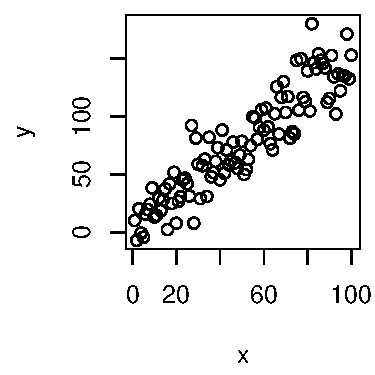
\includegraphics[bb=0in 0in 2.5in 2.5in, height=2.5in, width=2.5in]{Figure1.png}
    \label{fig:1}
\end{figure}

Hyperparameters optimization was done via Halving Grid Search, a successive halving algorithm that reduces the cost of optimization by exponentially decreasing the number of candidate models at each search iteration while increasing the resources and training cases given to each successful candidate \parencite{}
\end{document}

% \section{Results}
% Table~\ref{tab:BasicTable} summarizes the data. \lipsum[15]

% \begin{table}
%   \caption{Sample Basic Table}
%   \label{tab:BasicTable}
%   \begin{tabular}{@{}llr@{}}         \toprule
%   \multicolumn{2}{c}{Item}        \\ \cmidrule(r){1-2}
%   Animal    & Description & Price \\ \midrule
%   Gnat      & per gram    & 13.65 \\
%             & each        &  0.01 \\
%   Gnu       & stuffed     & 92.50 \\
%   Emu       & stuffed     & 33.33 \\
%   Armadillo & frozen      &  8.99 \\ \bottomrule
%   \end{tabular}
% \end{table}

% \begin{figure}
%     \caption{This is my first figure caption.}
%     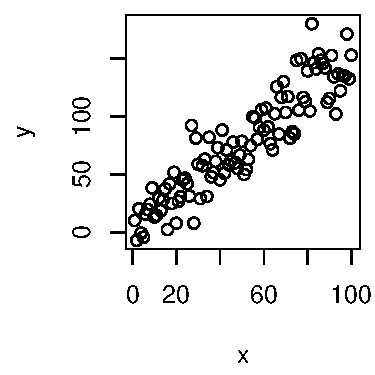
\includegraphics[bb=0in 0in 2.5in 2.5in, height=2.5in, width=2.5in]{Figure1.pdf}
%     \label{fig:Figure1}
% \end{figure}

% Figure~\ref{fig:Figure1} shows this trend. \lipsum[16]

% \section{Discussion}
% \lipsum[17]

% \lipsum[18]

% \lipsum[19]

% \printbibliography

% \appendix

% \section{Instrument}
% \label{app:instrument}

% As shown in Figure~\ref{fig:Figure2}, these results are impressive. \lipsum[20]

% \begin{figure}
%     \caption{This is my second figure caption.}
%     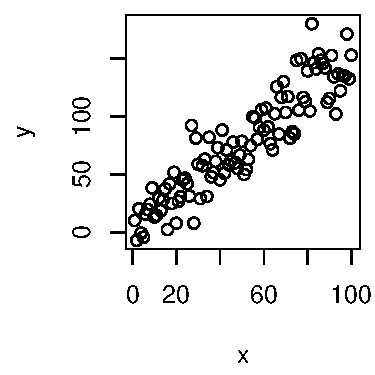
\includegraphics[bb=0in 0in 2.5in 2.5in, height=2.5in, width=2.5in]{Figure1.pdf}
%     \label{fig:Figure2}
% \end{figure}

% \lipsum[21]
% \section{Pilot Data}
% \label{app:surveydata}

% The detailed results are shown in Table~\ref{tab:DeckedTable}. \lipsum[22]

% \begin{table}
%   \begin{threeparttable}
%     \caption{A More Complex Decked Table}
%     \label{tab:DeckedTable}
%     \begin{tabular}{@{}lrrr@{}}         \toprule
%     Distribution type  & \multicolumn{2}{l}{Percentage of} & Total number   \\
%                        & \multicolumn{2}{l}{targets with}  & of trials per  \\
%                        & \multicolumn{2}{l}{segment in}    & participant    \\ \cmidrule(r){2-3}
%                                     &  Onset  &  Coda            &          \\ \midrule
%     Categorical -- onset\tabfnm{a}  &    100  &     0            &  196     \\
%     Probabilistic                   &     80  &    20\tabfnm{*}  &  200     \\
%     Categorical -- coda\tabfnm{b}   &      0  &   100\tabfnm{*}  &  196     \\ \midrule
%     \end{tabular}
%     \begin{tablenotes}[para,flushleft]
%         {\small
%             \textit{Note.} All data are approximate.

%             \tabfnt{a}Categorical may be onset.
%             \tabfnt{b}Categorical may also be coda.

%             \tabfnt{*}\textit{p} < .05.
%             \tabfnt{**}\textit{p} < .01.
%          }
%     \end{tablenotes}
%   \end{threeparttable}
% \end{table}

% \lipsum[23]

% \end{document}

% %%
% %% Copyright (C) 2019 by Daniel A. Weiss <daniel.weiss.led at gmail.com>
% %%
% %% This work may be distributed and/or modified under the
% %% conditions of the LaTeX Project Public License (LPPL), either
% %% version 1.3c of this license or (at your option) any later
% %% version.  The latest version of this license is in the file:
% %%
% %% http://www.latex-project.org/lppl.txt
% %%
% %% Users may freely modify these files without permission, as long as the
% %% copyright line and this statement are maintained intact.
% %%
% %% This work is not endorsed by, affiliated with, or probably even known
% %% by, the American Psychological Association.
% %%
% %% This work is "maintained" (as per LPPL maintenance status) by
% %% Daniel A. Weiss.
% %%
% %% This work consists of the file  apa7.dtx
% %% and the derived files           apa7.ins,
% %%                                 apa7.cls,
% %%                                 apa7.pdf,
% %%                                 README,
% %%                                 APA7american.txt,
% %%                                 APA7british.txt,
% %%                                 APA7dutch.txt,
% %%                                 APA7english.txt,
% %%                                 APA7german.txt,
% %%                                 APA7ngerman.txt,
% %%                                 APA7greek.txt,
% %%                                 APA7czech.txt,
% %%                                 APA7turkish.txt,
% %%                                 APA7endfloat.cfg,
% %%                                 Figure1.pdf,
% %%                                 shortsample.tex,
% %%                                 longsample.tex, and
% %%                                 bibliography.bib.
% %%
% %%
% %% End of file `./samples/longsample.tex'.
